% Document class
\documentclass[tikz, border = 0.05 cm]{standalone}

% TikZ packages
\usepackage{tikz}
\usepackage{tkz-euclide}
\usetikzlibrary{calc, patterns, angles, quotes, decorations.markings}

% Document
\begin{document}

% Tikz picture
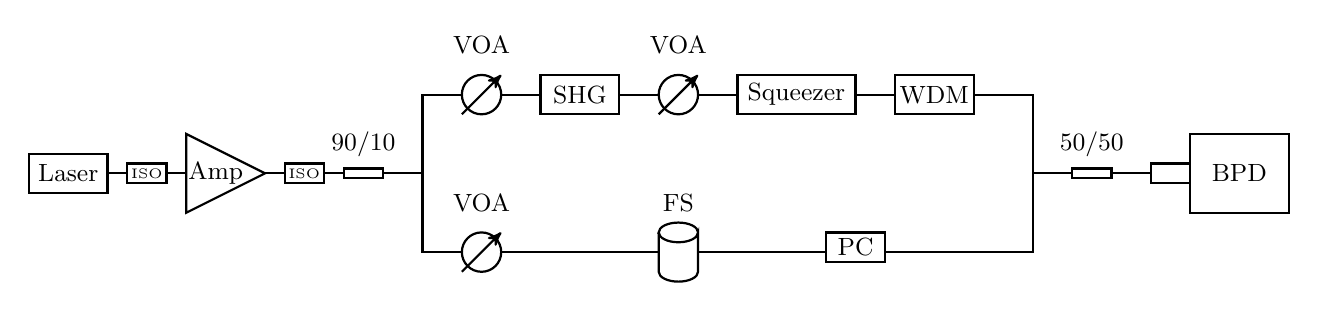
\begin{tikzpicture}
    % Upper segment of the cable
    \draw[thick] (+0.000, +0.000) -- (+5.000, +0.000) -- (+5.000, +1.000) -- (+12.750, +1.000) 
    -- (+12.750, +0.000) -- (+14.250, +0.000) -- (+14.250, +0.125) -- (+14.750, +0.125);

    % Lower segment of the cable
    \draw[thick] (+5.000, +0.000) -- (+5.000, -1.000) -- (+12.750, -1.000) -- (+12.750, +0.000);

    % Connection from the 50/50 to the BPD
    \draw[thick] (+14.250, +0.000) -- (+14.250, -0.125) -- (+14.750, -0.125);

    % === Elements from left to right ===
    % Laser
    \filldraw[thick, fill = white, draw = black] (+0.000, -0.250) 
    rectangle (+1.000, +0.250); \node at (+0.500, +0.000) {\small{Laser}};

    % ISO
    \filldraw[thick, fill = white, draw = black] (+1.250, -0.125) 
    rectangle (+1.750, +0.125); \node at (+1.500, +0.000) {\tiny{ISO}};

    % Amp
    \filldraw[thick, fill = white, draw = black] (+2.000, -0.500) -- (+2.000, +0.500)
    -- (+3.000, +0.000) -- cycle; \node at (+2.375, +0.000) {\small{Amp}};

    % ISO
    \filldraw[thick, fill = white, draw = black] (+3.250, -0.125) 
    rectangle (+3.750, +0.125); \node at (+3.500, +0.000) {\tiny{ISO}};

    % 90/10 splitter
    \filldraw[thick, fill = white, draw = black] (+4.000, -0.0625) 
    rectangle (+4.500, +0.0625); \node at (+4.250, +0.375) {\small{$90/10$}};

    % === Upper middle elements ===
    % VOA
    \filldraw[thick, fill = white, draw = black] (+5.750, +1.000) circle[radius = 0.25 cm]; 
    \node at (+5.750, +1.625) {\small{VOA}}; 
    \draw[thick, -stealth'] (+5.500, +0.750) -- (+6.000, +1.250); % Arrow

    % SHG
    \filldraw[thick, fill = white, draw = black] (+6.500, +0.750) 
    rectangle (+7.500, +1.250); \node at (+7.000, +1.000) {\small{SHG}};

    % VOA
    \filldraw[thick, fill = white, draw = black] (+8.250, +1.000) 
    circle[radius = 0.25 cm]; \node at (+8.250, +1.625) {\small{VOA}}; 
    \draw[thick, -stealth'] (+8.000, +0.750) -- (+8.500, +1.250); % Arrow

    % Squeezer
    \filldraw[thick, fill = white, draw = black] (+9.000, +0.750) 
    rectangle (+10.500, +1.250); \node at (+9.750, +1.000) {\small{Squeezer}}; 

    % WDM
    \filldraw[thick, fill = white, draw = black] (+11.000, +0.750) 
    rectangle (+12.000, +1.250); \node at (+11.500, +1.000) {\small{WDM}};
        
    % === Lower middle elements ===
    \filldraw[thick, fill = white, draw = black] (+5.750, -1.000) 
    circle[radius = 0.25 cm]; \node at (+5.750, -0.375) {\small{VOA}}; 
    \draw[thick, -stealth'] (+5.500, -1.250) -- (+6.000, -0.750);

    % FS
    \filldraw[thick, fill = white, draw = black] (+8.000, -0.750) -- (+8.000, -1.250)
    -- (+8.000, -1.250) arc (180: 360: 0.25 cm and 0.125 cm) -- (+8.500, -0.750)
    -- (+8.500, -0.750) arc(360: 180: 0.25 cm and 0.125 cm)
    -- (+8.000, -0.750) arc (180: 0: 0.25 cm and 0.125 cm); 
    \node at (+8.250, -0.375) {\small{FS}};

    % PC
    \filldraw[thick, fill = white, draw = black] (+9.875 + 0.250, -1.125) 
    rectangle (+10.625 + 0.250, -0.750); \node at (+10.250 + 0.250, -0.9375) {\small{PC}};

    %  === Right side ===
    % 50/50 splitter
    \filldraw[thick, fill = white, draw = black] (+13.000 + 0.250, -0.0625) 
    rectangle (+13.500 + 0.250, +0.0625); \node at (+13.250 + 0.250, +0.375) {\small{$50/50$}};

    % BDP
    \filldraw[thick, fill = white, draw = black] (+14.500 + 0.250, -0.500) 
    rectangle (+15.750 + 0.250, +0.500); \node at (+15.125 + 0.250, +0.000) {\small{BPD}};
\end{tikzpicture}

\end{document}
